\chapter{总结与展望}

\section{总结}
在本文中,为了解决医学图像中语义分割所需训练标签的高成本与难获取的问题,我们探索了弱监督语义分割的两个方向:基于弱标签和基于噪声标签的学习。

基于弱标签的语义分割只需要弱标注形式,本文为该任务提出了一种结合物体形状先验的弱分割模型与学习策略。本文的方法在模型训练与预测中充分利用形状先验,来弥补标签不足带来的分割性能下降。由于缺乏完整的物体形状,我们利用弱标签设计了一种自学习的形状表征,其中包括形状表征的选取、形状增强方法和形状去噪模型。语义分割模型和形状模型的结合,极大改进了训练过程和最终预测的效果。而迭代学习的策略,使得弱监督分割模型性能逐步提高并稳定收敛。
此外,本文设计了高效的稀疏弱标注策略,包含选择性标注和混合式标签,通过利用空间连续性和整体性,显著降低了标注成本,而尽可能保留弱标签的信息量。
两个不同的数据集上(气管和前列腺)的实验结果表明,本文的方法在多种弱标注设定下都取得了最高的性能,并且表现出良好的鲁棒性。在可视化结果的对比上,我们的分割结果具有更干净完整的形状,证明了本文方法对物体形状的改进效果,以及形状先验在弱监督语义分割中的重要作用。

基于噪声标签的语义分割的核心问题,是充分利用正确标签的信息,而减少错误标签对训练的干扰。为此,本文利用图像的结构先验和像素标签的相关性,提出一种结合超像素表征的鲁棒学习策略。
超像素表征能使我们在分割标签上施加结构约束,并且尽可能保留物体的边缘信息。而基于超像素表征的模型学习,可以更准确地选择可靠的正确标签参与训练,并纠正不可靠的标签。在训练策略上,本文提出了有噪声感知的网络更新和标签更新交替进行的迭代学习,充分利用了标签的有效信息并不断更新改进。
本文所提的方法在两个数据集的四种类别上进行实验,结果表明本文方法超越了之前的工作,有着优异的分割性能,并保持了训练的稳定收敛。多种噪声水平设定下的数值变化表明,本文方法具有较强的鲁棒性和泛化性能。此外,我们的预测结果更接近真实完整的物体边缘。

\section{展望}
在上述两个方向的探索过程中,我们发现了一些值得进一步研究的问题。

在基于弱标签的语义分割中,预测结果中有一些误差较大的案例,如图~\ref{fig:failure}所示。它们表现为不完整的或过多的预测掩膜,即使其输入图像在像素强度或边缘都比较明显。
这主要是因为我们的模型是在弱标签上训练,而没有在训练中结合物体边缘信息或约束。针对这样的问题,可以考虑在模型中加入图像的低阶特征,比如边缘特征或超像素等,来进一步改善。
    \begin{figure}[tbp]
        \centering 
        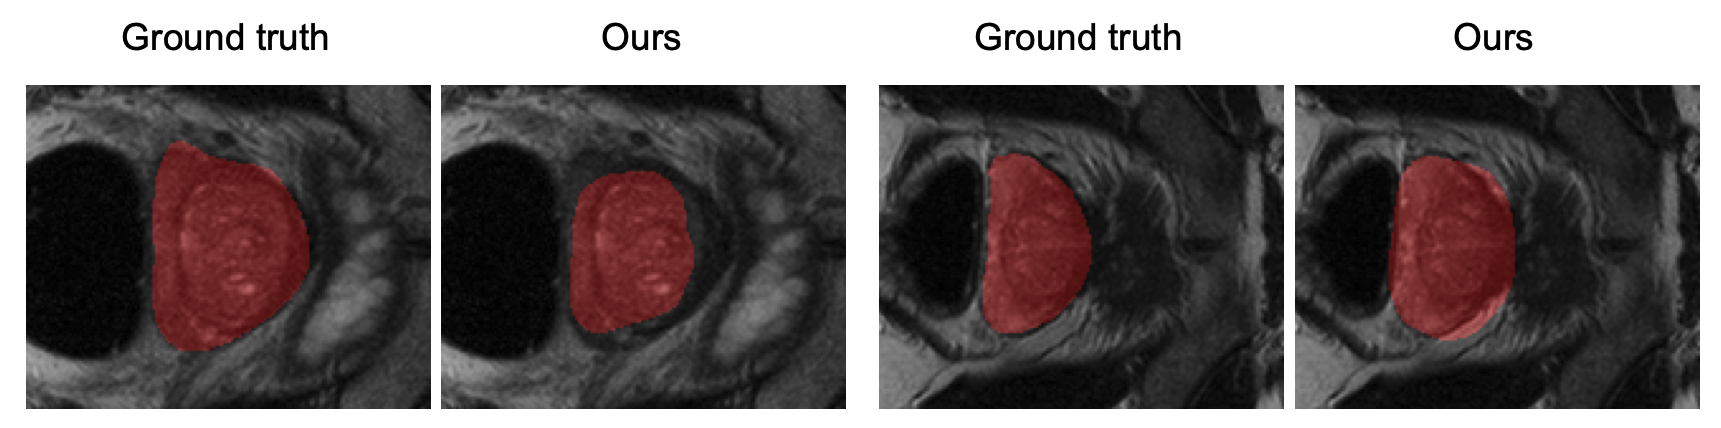
\includegraphics[width=1.0\textwidth]{img/c3/f51m.png}
        \bicaption{两个在前列腺数据集的失败的预测案例。}
        {Two failure cases on prostate dataset.}
        \label{fig:failure}
    \end{figure}

另外,由于多数医学图像的目标分割器官都有较大的相似性,我们的方法实际上捕捉了一类相近的形状表征。但真实世界中也有很多其他类别的物体,它们具有较大的形状差异。当这些物体无法仅用一类形状来表示,而呈现出多类或者层次结构的形状时,本文的方法就需要进行拓展。具体而高效的形状模型需要更多探索。更进一步,现有的形状模型有大量的参数,训练需要较长时间而部署也需要较大内存,能否降低形状模型的复杂度,或者将其与语义分割模型深度地结合,是很有研究价值的方向。

在基于噪声标签的语义分割中,超像素质量和真实噪声数据集值得进一步关注。
我们的基于超像素表征的鲁棒学习方法被证明是有效的,并且具有较好的泛化性。但是,超像素的生成质量仍有一些误差,这些误差一定程度上限制了方法效果的进一步提升。
现有的离线生成方法(如 SLIC)改进空间不大,如何自适应地生成更准确的超像素或者更广泛的感知表征,具有十分重要的意义。
同时,在更广泛的应用场景,比如同一图像中不同尺寸的目标物体,如何基于图像结构先验设计高质量的表征方法,值得深入探索。

在数据集层面,由于缺少具有真实噪声标签的公开数据集,我们使用模拟的标签噪声作为替代。虽然探索了膨胀、腐蚀等形态学和仿射变换噪声模式,真实的标签噪声可能呈现更多样更细节的变化。为了所提方法的可用性和泛化性,探索真实世界的噪声标签处理是一个重要的问题。只是收集这样一个数据集需要耗费大量的资源,因此作为未来的一个探索方向。